\section{ISO-OSI, TCP/IP}
\label{sec:isoosi}
\subsection{ISO-OSI}
Problematika komunikace po síti byla tak široká, že vznikl mezinárodní refernční standard, který ji popisuje vrstvovým modelem.
Tento standard nespecifikuje realizaci, pouze její normy.
Má 7 vrstev: \\
\begin{tabularx}{\linewidth}{l|l|l|l}
  \textbf{Pořadí} & \textbf{Název} & \textbf{Data} & \textbf{Pozn.}                                                            \\
  \hline
  1.              & Aplikační      & Message       & Formátuje data pomocí protokolů (HTTP, SSH, FTP, DNS, DHCP, POP3)         \\
  \hline
  2.              & Prezentační    & Data          & Reprezentuje data a zabezpečení aplikacím (Kódování, komprese, šifrování) \\
  \hline
  3.              & Relační        & Rel. packet   & Zabezpečuje začátek a konec spojení, výměnu, integritu a korektnost dat   \\
  \hline
  4.              & Transportní    & Segment       & Zajišťuje předání paketů správné aplikaci                                 \\
  \hline
  5.              & Síťová         & Packet        & Přenos dat mezi vzdálenými počítači. Komunikace pomocí IP                 \\
  \hline
  6.              & Linková        & Frame         & Logické spojení na úrovni LAN. Komunikace pomocí MAC                      \\
  \hline
  7.              & Fyzická        & Bit           & Fyzické spojení stran (Kabely, HW, konektory \dots)                       \\
\end{tabularx}
Komunikace mezi dvěma počítači je nutné z prvního počítače vést ze sedmé vrstvy do první a následně na druhém z první vrstvy do sedmé.
\subsection{TCP}
TCP/IP je skupina protokolů pro komunikaci používané např. na internetu.
Má za úkol zajistit možnost propojení sítí založených na různých technologií.
Zajistit vysokou přenosovou rychlost na úkor spolehlivosti, jelikož o tu se starají koncové uzly již sami.
\begin{multicols}{2}
  Komunikace na TCP probíhá na: \\
  \begin{enumerate}
    \item Aplikační vrstvě
    \item Transportní vrstvě
    \item Síťové vrstvě
    \item Vrstvě síťového rozhraní
          \begin{enumerate}
            \item Fyzické vrstvě
            \item Logické vrstvě
          \end{enumerate}
  \end{enumerate}
  \columnbreak
  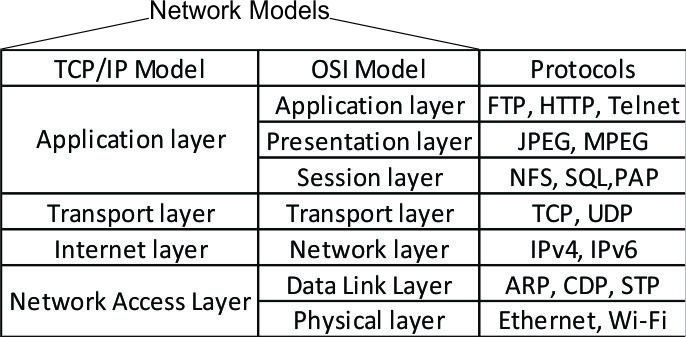
\includegraphics[height=4cm]{TVY-POS/ISO-OSI-TCP-IP/tcpip.jpg}
\end{multicols}
V koncových uzlech jsou implementovány všechny vrstvy pro kontrolu dat, v přechodových uzlech je implementována pouze síťová vrstva a vrstva síťového rozhraní.
Komunikace probíhá mezi sousedními vrstvami nebo mezi stejnolehlými vrstvami.
Pro komunikaci se používá buďto TCP, nebo UDP.
\subsection{IP}
Univerzální přenosový protokol k nespolehlivému, nespojovanému přenosu dat mezi zdrojovým počítačem a příjemcem.
Každé zařízení dostává nějakou indentifikaci v podobě IP adresy.
Přenášená data se nazývají IP datagramy neboli IP pakety, každý paket obsahuje hlavičku, ve které nese metadata a vlastní přenášená data.
Dnes se používají protokoly IPv4 a IPv6.
Cesta není předem vytyčena a optimální cestu nachází každý uzel, přes který daný paket jde.
Zpráva rozdělená na několik paketů nemusí dorazit ve stejném pořadí, jako byla poslána.
Každý poškozený paket síťová vrstva zahodí.
Požaduje-li aplikace spolehlivý přenos dat, jsou k dispozici protokoly vyšších vrstev.
Při přenosu velkých dat se mohou data fragmentovat.
Fragmentují se na vysílající stanici a defragmentují na přijímací.
\subsection{IEEE}
Jedná se o mezinárodní institum zabývající se výrobou standartů v oblasti internetového průmyslu.
Jejich protkoly se používají pro spoustu řešení v této problemice.
Od protokolu 802.1q pro trunk komunikaci ve VLAN až po 802.11 pro specikiaci WI-FI technologie.
